\documentclass[oribibl]{llncs}
 
\usepackage{amssymb} % AMS Fonts
\usepackage{amsmath} % AMSLaTeX
\usepackage{url}
\usepackage[pdftex]{graphicx}

% Compile only with pdfLaTeX
\usepackage[pdftex]{graphicx}

%\reversemarginpar
\makeatletter
\@twosidefalse
\makeatother

\textwidth180mm
\hoffset-30mm

\bibliographystyle{alpha}

\begin{document}

\title{ Skip Lists, Jump Lists, and Other Randomized Data Structures for Maintaining Ordered Sets}

\author{Bairong Lei, Michael Wexler}

\institute{University of Waterloo, David R. Cheriton School of Computer Science}

\maketitle

\begin{abstract}
  In this project, we will discuss several probabalistic data structures for maintaining ordered sets. These
  data structures use probabalistic methods to keep balanced, which helps to avoid skewed distributions that
  can lead to excessive running times. 
\end{abstract}

%%%%%%%%%%%%%%%%%%%%%%%%%%%%%%%%%%%%%%%%%%%%%%%%%%

\section{Introduction}

The need for ordered sets is very common in computer science. By ordered set, we mean a typical set data structure which has the additional property of maintaining the order of its elements. Programmers often need
such a structure in order to determine if a given element is in the set, and also to find the nearest predecessor for a given element. Given the functionality of an ordered set, it can be extended so that every 
key maps to a certain value. This would essentially be a dictionary data structure. One would hope that the most common dictionary operations would take O(log n), or better yet, O(1) time.

There has been much work in developing set data structures that provide O(log n) lookup time. Examples of these are hash-tables, AVL trees, and red-black trees. In addition to quick lookup times, AVL trees and red-black trees have the additional property of being able to provide O(log n) time for the next-predecessor operation, which, for a given key, will give the smallest key that is greater than that key.

For the afforementioned dictionary data structures, there is often the occurence where 

For instance, for a given n, if we were to insert the sequence 1 2 ... n into a normal binary search tree, we would end up having a very skewed structure, which would could take O(n) time to find an element. This is the reason AVL and red-black trees were developed. They use deterministic methods to perform self-balancing, so the skewed distribution never occurs.

The afforementioned data structures in their classical implementations all use deterministic methods for organizing their data.  Oftentimes, one wants to put a certain element of randomness into their dictionary data structures in order to avoid situations where their data structure becomes skewed. In this paper we will discuss various data structures that use randomness in order to maintain a level of balance, to avoid skewed distributions.

This paper is organized as follows: section \ref{sctn:randomized_data_structures} will give an overview on several probabalistic set data structures. Section \ref{sctn:experiments} will give an overview on some experiments we performed in order to compare these data structures.

The last section draws a conclusion of our work.

All test files and program code we describe in this report can be found in our \textsc{GitHub} repository \url{https://github.com/wexlermi/cs840project}.

%%%%%%%%%%%%%%%%%%%%%%%%%%%%%%%%%%%%%%%%%%%%%%%%%%

\section{Randomized data structures}
\label{sctn:randomized_data_structures}

\subsection{Treaps}
The first randomized data structure we will discuss is the treap \cite{Aragon1989}. Treaps are at their foundation binary-search-trees, with a certain amount of randomness that allows them to remain balanced in the average case. Every element in a treap has the binary-search-tree property, such that all the nodes in its right subtree are greater than the root, and all the nodes in its left subtree are less than the root. However, every node in a treap contains a priority value, in which the priority of a treap node is always higher than that of its children. When we insert a new element into the treap, we randomly assign it a priority, which is a random integer from a sufficiently large range to ensure there are no collisions. Then we put the element in the treap, in the place it would go if it were considered only as a binary search tree. Once it is put in its proper place in the treap, a sequence of rotations are performed to restore the priority requirement, while still maintaining proper place to make sure its key is in the proper order.

\begin{figure}[here]
\center
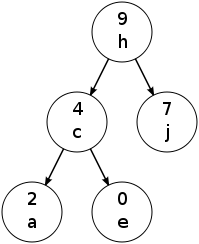
\includegraphics[width=7cm]{images/treap}
\caption{Example of a treap from http://en.wikipedia.org/wiki/File:TreapAlphaKey.svg}
\label{fig:treap}
\end{figure}

Figure \ref{fig:treap} is an example of a very small treap. The letters represent keys, and have the in-order property one would expect in a binary search tree. The numbers represent the priorities. In this case we have a max-heap, since each node has a priority which is a number greater than its children.

\subsection{Skip lists}
A skip-list \cite{skip_list} is a randomized data structure that is inherently built upon linked-lists. Imagine we had a linked list of $n$ numbers, in sorted order. If we had to search for an element $x$ in this linked-list, it would be quite inefficient to linearly search for it. To resolve this issue, we can put pointers every other element, or every 3rd element, etc. This way, when searching for an element, we can first search through the top level, and once we find an element greater than it, we can drop down and search our original linked list.

We can repeat the process for the top linked list: put pointers to every other element. We keep repeating this process, where each higher level has half the pointers of the level below it, until we get a level which has 1 or 2 pointers. Then when we search for an element x, we start at the top list, skipping over elements that are less, then dropping down to lower and lower levels, repeating the process, until we either find the element we are looking for, or reach the bottom level and overshoot it, in which case we determine that the element does not exist in the skip list.

Skip-lists use probabalistic methods in order to determine how many levels of a skip-list a given element can be found on.. We specify a varible $p$ which represents the probability that an element on level $i$ will appear on level $i+1$. Every element appears on level 0, as we go to higher levels, we will find less and less elements. The typical value is $p=\frac{1}{2}$. Every time we would like to insert a key $x$ into the skip-list, we first put it at level 0. Then, we "flip a coin" a certain amount of times, and while we are getting heads, we keep adding the element to higher and higher levels, until we get a tails, and then we stop. This will mathematically ensure that our skip-list has approximately half the number of nodes at higher and higher levels.



\begin{figure}[here]
\center
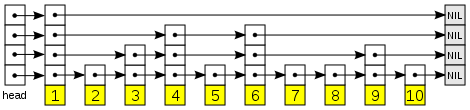
\includegraphics[width=7cm]{images/skip_list}
\caption{Example of a skip-list from \cite{skip_list}}
\label{fig:skip_list}
\end{figure}

\begin{figure}[here]
\center
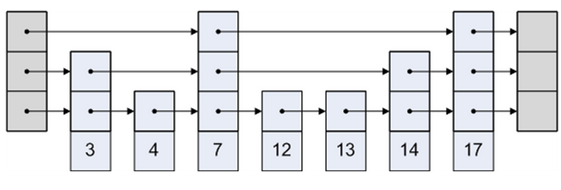
\includegraphics[width=7cm]{images/skip_list1}
\caption{Example of a skip-list}
\label{fig:skip_list}
\end{figure}

\subsection{Skip lifts}

In \cite{skip_lift} Bose, Douïeb, Morin talk about an improvement to the skip list called the skip lift. A skip lift is a skip list in which every element only has the top two nodes. The rest are deleted. This greatly reduces the size of the skip list.

\begin{figure}[here]
\center
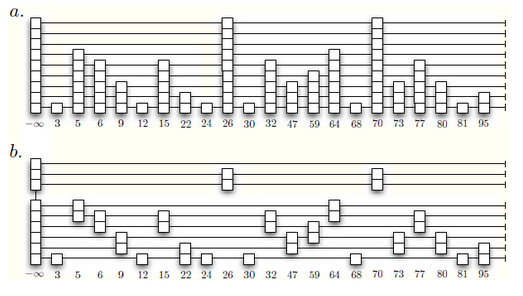
\includegraphics[width=12cm]{images/skiplist_vs_skiplift}
\caption{Skip-list (a)  vs. skip-lift (b)}
\label{fig:skip_list}
\end{figure}


\subsection{Jump lists}

Jump-lists \cite{jump_list} are sorted linked-lists, in which case search is expedited by putting "jump" pointers on several nodes, which serve as an "express-lane" for searching. During the course of this project, we came across three variations of the jumplist data structure. These three types of jumplists differ by their methods of establishing the jump links for each node in the list. In the original paper \cite{jump_list}, a jumplist is a sorted single or double linked list. This linked list is a circular linked list with an empty value header. Each node has a key value and a next pointer to connect its immediate successor. Meanwhile, each node has a jump pointer that enables it to jump over several of its successors to reach one of its successors. The link between a node and the target node its jump pointer points to is known as an arch. The arch of the header node of the jumplist is called the {\it fundamental arch}. The jump pointers are created as follows: The node pointed by the jump pointer of the header of the list is selected randomly amongst the rest of the nodes of the list. This assignment splits the list into two independent sublists which are built recursively using the same random procedure. During this construction, the jump pointers do not cross each other. Each node of this jumplist can have more than one incoming jump pointers, but have only one jump pointer pointing to its successor.

The second variation of the jumplist data structure is found in \cite{skip_lift}. It has most of the same features as the jumplist featured in \cite{jump_list}. It maintains the core feature that the jump pointers do not cross over each other. Meanwhile, it ensures that each node has at most one jump pointer being pointed to it and only one jump pointer pointing to its successor. Figure \ref{fig:jumplist} depicts a sample randomized jumplist with 21 nodes.


\begin{figure}[here]
\center
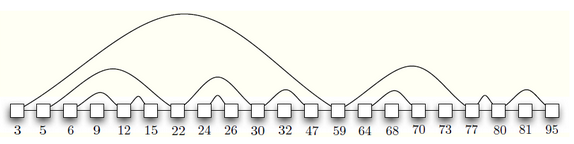
\includegraphics[width=15cm]{images/jumplist}
\caption{A randomized jumplist with 21 nodes}
\label{fig:jumplist}
\end{figure}


The third variation of the jumplist data structure comes from \cite{ElmasryMarch2005}. Like the jumplist introduced by the original randomized jumplist paper, its jumplist maintains the set of common features such as the fact that jump pointers can not cross over each other. However, when the jump pointers are created for the jumplist, the procedure first selects the median node as the node pointed by the jump pointer of the jump list. This fundamental arch divides the whole list into two sublists evenly. These two sublists are then further split evenly and independently using the same process until it reaches the smallest sublists that have only one node and make its jump pointers point to itself. This process builds what they refer to as a {\it perfect jumplist}. Figure \ref{fig:jumplist} depicts an example of a perfect jumplist with 23 elements.


\begin{figure}[here]
\center
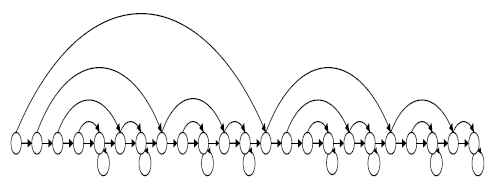
\includegraphics[width=12cm]{images/perfect_jumplist}
\caption{A perfect jumplist with 23 elements}
\label{fig:jumplist}
\end{figure}


\subsubsection{Supported methods:}

A jumplist usually has a set of common methods that a dictionary data structure contains. Search, successor, insertion and deletion are the most popular methods a dictionary data structure supports. Our project aims to implement some of these methods for the jumplist data structure, evaluate and verify its theoretical running time estimation suggested from the Deterministic jumplists paper.

Implementation:

There are some challenges to implement the insertion and deletion methods for the jumplist, since the pseudo code for these two methods are missing in the original randomized jumplist paper. Although there has been a C plus plus implementation for the jumplist data structure in H. Brönnimann’s research work (\url{http://photon.poly.edu/~hbr/publi/jumplist.html}) from the Polytechnic University, unfortunately its source code is too old and severely handicapped for its missing search and insertion methods so that we have to pursure another solution. Another challenge is when we strive to use the insertion algorithm from the deterministic jumplist paper, we find there is a defect in that algorithm so that whenever there is an inserted item whose value is less than the value of the header node, the insertion method always places it to the second place of the list.

We decide to implement our data structures in Java. For the time being, we only implement the search and insertion methods for the jumplist. The jumplist is initialized as an ordinary linked list at the beginning. A method called buildperfectjumplist is invoked to create the jump pointers for each node using the algorithm introduced in the deterministic jumplist paper. Meanwhile, each node updates its corresponding sizes of its next and jump sublists. The search method is implemented basing on its algorithm in the randomized jumplist paper to use the jump links as many as possible to skip nodes to speed up the search. For the insertion method we have implemented two versions to compare their running time. The first insert method is called djinsert which uses exactly the same algorithm introduced in the deterministic jumplist paper and inherits the first item insertion defect stated previously. After a new item is inserted, its jump pointer is updated as follows: The whole list is iterated to check whether there exists a node violating the balancing condition to rebuild the jump pointers for the entire list. If the jump pointer of the predecessor of the new item points to itself, its jump pointer is changed to point to the new item and the new item also inherits the jump pointer of its immediate successor. Meanwhile, the new item’s sizes of its next and jump sublists is updated respectively. On the other hand, the other insertion method follows the basic search algorithm to find the insertion point and inserts the new item as well as calling the buildperfectjumplist method to rebuild all the jump pointer for the entire list. This method resolves the first item insertion defect and does not need to maintain its sizes of next and jump sublists, but we expect the its running time is longer due to the redundancy of its jump pointer rebuilding procedure.

Running result:


\subsection{Skynet}

Skynet is a scalable overlay network designed to eliminate the disadvantages of peer-to-peer systems that have no control of data storage location and do not satisfy the need to restrain the routing path within a certain range. Due to time constraints, we were unable to implement SkyNet, but instead we will give a brief overview of the purpose and design of SkyNet.

\begin{figure}[here]
\center
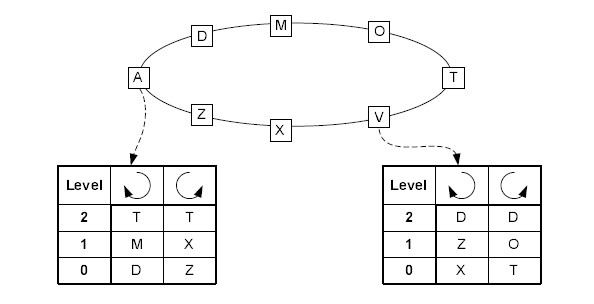
\includegraphics[width=12cm]{images/skynet}
\caption{A Skynet with 8 elements}
\label{fig:skynet}
\end{figure}

Essentially, the structure of the Skynet is a circular double linked list. Each of node of this ring structure has a name ID field which is known as the data record key. From Figure \ref{fig:skynet}, we can see a Skynet structure \cite{skip_net} with eight nodes, each of which has an alphabetic character. Each Skynet node store $2\log{N}$ pointers, where $N$ is the number of nodes in this structure. The pointers facilitate a set of rings as paths for routing through nodes in the rings to search an item. Figure \ref{fig:skynet1} demonstrates the same Skynet of Figure \ref{fig:skynet}, which shows a diverse set of rings by selecting nodes of every level to establish interconnections. For example, from the root ring, we may choose nodes of A, M, T and X to form a subring for the level 1 overlay. We may also further select nodes of A, T and M, X to form two subrings for level 2 overlay from its upper level ring. We continue to use this process to form smaller and smaller subrings until each node only has itself as the new ring. Meanwhile, each node is assigned a numeric ID representing the routing path to reach it.

\subsubsection{Routing in the SkyNet:}

Routing can follow a clockwise direction or a counter-clockwise direction. There are two routing approaches to support lexicographic searching. One approach is called {\it Routing by name ID}. For example, if we need to search node V from node A, this methodology begins routing from Ring 00. Since there are only nodes A and T in Ring 00, it goes down one level to level 1 to route around the subring formed with nodes A, M, T and X. At this moment, we can find node V, so it goes down one level to the level 0 to route around the root ring and eventually find the node V. Another routing approach is called {\it Routing by numeric ID}. There is a hash function that transfers the key of the target item into its corresponding numeric ID. Using the same example to search for node V, the hash function transfers the key V into 111. Therefore, to search node V from node A, the first digit of the numeric ID 111 is 1 and guides the routing from the root ring to the right subring Ring 1 in level 1. Then the second digit 1 directs the routing to the right subring Ring 11 in level 2. Eventually the last digit 1 guides the search routing to the right subring Ring 111 in level 3 and find the target node V. The run time for both Routing by name ID and numeric ID is $O(\log{n})$, where $n$ is the number of the nodes.  Potential future work for this structure can be implementing the insertion and deletion methods.

\begin{figure}[here]
\center
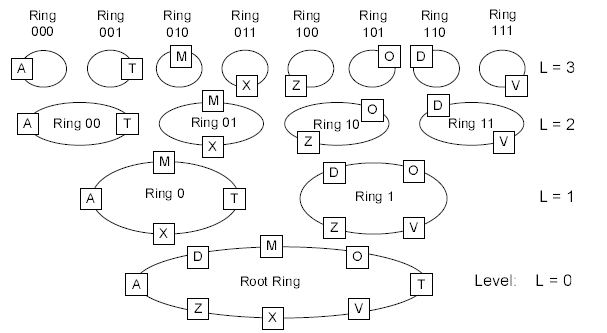
\includegraphics[width=12cm]{images/skynet1}
\caption{A ring hierarchy for an 8-node Skynet}
\label{fig:skynet1}
\end{figure}


\section{Implementation}
\label{sctn:implementation}

For this project, we decided to implement the skip lift \cite{skip_lift}. We built our implementation off an implementation of the skip list \cite{skip_list_imp}. We also implemented the jump list\cite{jump_list}.  Our implementations can be found on our GitHub here: \url{http://github.com/wexlermi/cs840project}.

 \section{Experiment and Analysis}
\label{sctn:experiment}

We thought it would be interesting to collect metrics on runtime and datasize of these data structures, to see which ones perform most competitively from a time and space performance perspective.

For our experiment, we generated a test data set of one million randomly chosen integers. For each of our data structures, we measured the timing it would take to insert all the test data into the data structure, as well as the space occupied in memory of the data structure. Also, we made a random permutation of the elements in our data set, which represents a sequence of requests. For this sequence of requests, we measured the time it took to query all the elements for each data structure.


\begin{table}[htbp]
\caption{Timings for each data structure in milliseconds}
\begin{center}
\begin{tabular}{|r|r|r|r|r|r|}
\hline
Data Structure & Time to insert & Time to query \\ \hline
AVLTree & 0.75 & 0.75 \\ \hline
Treap & 0.75 & 0.75\\ \hline
SkipList & 0.667 & 0.667  \\ \hline
SkipLift & 0.625 & 0.75  \\ \hline
JumpList & 0.6 & 0.7 \\ \hline
\end{tabular}
\end{center}
\label{abc}
\end{table}

\begin{table}[htbp]
\caption{Space occupied by the data structures}
\begin{center}
\begin{tabular}{|r|r|r|r|r|r|}
\hline
Data Structure & Space (megabytes) \\ \hline
AVLTree & 0.75 \\ \hline
Treap & 0.75\\ \hline
SkipList & 0.667   \\ \hline
SkipLift & 0.625  \\ \hline
JumpList & 0.6 \\ \hline
\end{tabular}
\end{center}
\label{abc}
\end{table}

We conjectured that the skip lift would take less space than the skip list.


\begin{remark}
Hello
\end{remark}

\begin{itemize}
  \item The executable file that was compiled by \texttt{crestc}
  \item A number of maximal iterations through the control flow graph
    we want to allow (i.e. a limitation to the paths we
    want to consider. Otherwise the program might run too long)
  \item A strategy \textsc{CREST} should use to traverse the control
    flow graph. Possible options here are in the set
\begin{center}
$\{$\texttt{dfs}, \texttt{cfg}, \texttt{random},
    \texttt{uniform\_random}, \texttt{random\_input}, 
    \texttt{cfg\_baseline}, \texttt{hybrid}$\}$
\end{center}
\end{itemize}



\section{Conclusion and Future Work}
\label{sctn:Conclusion}

There are several conclusions we can draw in this report.


\bibliographystyle{plain}
\bibliography{report}

\end{document}
